\documentclass{bredelebeamer}
\usepackage{graphicx}
\usepackage{amsmath,amsfonts,amsthm}
\usepackage{hyperref}
\usepackage{setspace}
\usepackage{makecell}
%\usepackage{media9} % for movies
%\usepackage{multimedia} % for movies
\usepackage{caption} % for figure caption
\usepackage{animate}
\usepackage[final]{listings} % for listing source code
\usefonttheme[onlymath]{serif} % make the equations look better
% define box for listing
\definecolor{myblue}{HTML}{4C72B0}
\definecolor{myred}{HTML}{C54E52}
\definecolor{mygreen}{HTML}{56A968}
\lstset{
      language=C++,
      basicstyle=\ttfamily,
      frame=single,
      columns=flexible,
      breaklines=true,
      showstringspaces=false,
      commentstyle=\color{mygreen},
      keywordstyle = \color{myblue},
      stringstyle  = \color{orange},
      }
\usepackage[absolute,overlay]{textpos} 
\setlength{\parskip}{0.9em}
\setbeamertemplate{navigation symbols}{}
\newcommand*\dif{\mathop{}\!\mathrm{d}}
%%%%%%%%% some settings
\captionsetup[figure]{labelformat=empty} % remove the prefix 'figure' for figure caption
\captionsetup[table]{labelformat=empty} % remove the prefix 'table' for figure caption
\setbeamertemplate{headline}{} %%%%%%%%%%% remove header %%%%%%%%%%%
\setbeamerfont{frametitle}{size=\Large} %% title font size
\renewcommand{\arraystretch}{1.5} % line space in a table
%%%%%%%%%% title
\title[ ]{DAFoam Workshop 2025}
\subtitle{v4.0.2}

\author{Ping He\\ ~ \\August 14, 2025 }


\date[August 14, 2025]{}

\setbeamercolor{title}{fg=Black,bg=White!0}
\setbeamercolor{frametitle}{fg=Black,bg=White!0}
%gets rid of footer
%will override 'frame number' instruction above
%comment out to revert to previous/default definitions
\setbeamertemplate{footline}[page number]

\begin{document}

%---------------------------------------------------------------%
\begin{frame}
  \titlepage
\end{frame}

%---------------------------------------------------------------%


%---------------------------------------------------------------%
\begin{frame}{Objectives}

After this workshop, you should be able to
\begin{itemize}
  \setlength\itemsep{1em}
 \item Identify the new APIs in runScript.py in DAFoam v4
 \item Get familiar with the new code structure in DAFoam v4 
 \item Run tutorials and add new features to DAFoam v4
\end{itemize} 

\end{frame}
%---------------------------------------------------------------%


%---------------------------------------------------------------%
\begin{frame}{Outline}

\textbf{Part 1: User-Focused Features}
\begin{itemize}
  \setlength\itemsep{1em}
 \item Overview of new run scripts, APIs, and solver options
 \item Walkthrough of selected tutorials
\end{itemize}

\textbf{Part 2: Developer-Focused Updates}
\begin{itemize}
  \setlength\itemsep{1em}
 \item Introduction to the updated code structure
 \item Examples of extending DAFoam (e.g., adding new design variables)
\end{itemize}

Note: We assume you are familiar with DAFoam v3 and will mainly focus on the new features in v4.

\end{frame}
%---------------------------------------------------------------%

%---------------------------------------------------------------%
\begin{frame}{}

  \begin{center}
     \noindent \Large{Part 1: User-Focused Features}
  \end{center}

  \begin{center}
    \noindent \large{Objective: let the DAFoam APIs be more consistent with the OpenMDAO standard.}
 \end{center}
  
  \end{frame}
  %---------------------------------------------------------------%


%---------------------------------------------------------------%
\begin{frame}{New interfaces in v4 runScript.py}

DAFoam v2 scripts are completely deprecated, but v3 scripts can be used with minor changes. Let us compare runScript\_v3.py and runScript\_v4.py in examples/NACA0012

\begin{itemize}

  \item The \texttt{-task} flag is changed to be consistent with OpenMDAO
  \item \texttt{objFunc} is replaced with \texttt{function} in \texttt{daOption}.
  \item \texttt{addToAdjoint} is no longer needed in \texttt{function}.
  \item \texttt{alphaName} is replaced with \texttt{patchVelocityInputName} for the angle of attack definition for force (e.g., CD and CL) \texttt{function}.
  \item \texttt{designVar} is replaced with \texttt{inputInfo} in \texttt{daOption}.
  \item The aoa function is defined in \texttt{inputInfo} instead of \texttt{configure}
  \item A new way to define shape for 2D airfoil using \texttt{non\_addShapeFunctionDV}.
\end{itemize}

\end{frame}
%---------------------------------------------------------------%

%---------------------------------------------------------------%
\begin{frame}{Details of the new \texttt{inputInfo} key in \texttt{daOptions}}

  \texttt{inputInfo} defines the input variables for a component in OpenMDAO. Let us check runScript\_test\_inputInto.py in examples/NACA0012
  
  \begin{itemize}
  
    \item Each key in \texttt{inputInfo} defines an input variable for a component, specified by the \texttt{components} key. Note: one input can be connected to multiple components.
    \item The name of the key in \texttt{inputInfo} is the name of the input for that component. Run the script and check the N2 diagram in mphys\_n2.html.
    \item The \texttt{type} key defines the type of this input. Check all available input types from examples/dafoam-4.0.2/src/adjoint/DAInput/*.H
    \item Each input type has its own customized keys, such as \texttt{patches}, \texttt{fieldName}, and \texttt{distributed}.
    \item Once an input is defined in \texttt{inputInfo}, we can connect dvs.output to it. Check line 163 in runScript\_test\_inputInto.py
    \item NOTE: Carefully define the inputs to avoid conflicts!
  \end{itemize}
  
  \end{frame}
  %---------------------------------------------------------------%


%---------------------------------------------------------------%
\begin{frame}{New interfaces for MDO problems}

  Let us comopare runScript\_v3.py and runScript\_v4.py in examples/MACH\_Tutorial\_Wing
  
  \begin{itemize}
  
    \item The \texttt{couplingInfo} key is deprecated, and the MDO coupling is now defined in \texttt{inputInfo} and \texttt{outputInfo}.
    \item The aerostructural problem has a \texttt{forceCoupling} component, which replaces the \texttt{getForce} component in v3. This component uses the volume coordinates and states as input and outputs the surface force (f\_aero). So we need to define this f\_aero as the output in \texttt{outputInfo}. 
    \item The \texttt{forceCouplingOutput} type in \texttt{outputInfo} will tell mphys\_dafoam that we have an aerostructural problem, and it will then trigger the aero-structural related codes in mphys\_dafoam.py.
    \item The \texttt{forceCoupling} component will automatically get the volume coordinates and states from the solver component, so we don't need to manually define these inputs in \texttt{inputInfo}.
    
    
\end{itemize}
\end{frame}
%---------------------------------------------------------------%

%---------------------------------------------------------------%
\begin{frame}{New interfaces for unsteady problems}

   Let us check runScript.py in examples/Cylinder
  
  \begin{itemize}
  \item We treat the unsteady flow/adjoint solver as an explicit component in OpenMDAO (line 116).
  \item The inputs for this explicit component are defined by \texttt{add\_design\_var} and the outputs are defined in \texttt{unsteadyCompOutput}. Here, each key (e.g., obj) in \texttt{unsteadyCompOutput} is the actual function used in optimization. Their sub-keys (e.g., CD and CL) are the functions defined in \texttt{daOption-function}. If one defines more than one sub-key, these functions will be added together.  
   \item Define unsteady adjoint-related parameters in \texttt{unsteadyAdjoint}.
   \item All components are promoted, so you should directly use \texttt{shape}, instead of \texttt{dvs.shape}.
    
\end{itemize}
\end{frame}
%---------------------------------------------------------------%


%---------------------------------------------------------------%
\begin{frame}{}

  \begin{center}
     \noindent \Large{Part 2: Developer-Focused Updates}
  \end{center}

  \begin{center}
    \noindent \large{Objective: make the DAFoam development easier.}
 \end{center}
  
\end{frame}
%---------------------------------------------------------------%

%---------------------------------------------------------------%
\begin{frame}{Improvements in DAFoam v4 development}

\begin{table}
\centering
\begin{tabular}{ccc}
\hline
& v3 & v4 \\
\hline
First build time & $>$30 mins & $\sim$10 mins \\
Re-build time & $>$30 mins & $\ll$10 mins \\
Build command & Multiple commands & One command \\
Parallel build & Fixed 4 cores & Max available cores \\ 
DAFoam libs &  Three libs (e.g., incomp) & One lib \\
Add new DVs & Multiple new functions & One new function \\
Add new partials & Ad-hoc & Standardized \\
Add new in/out & Ad-hoc & Standardized \\

\hline
\end{tabular}
\end{table}

\end{frame}
%---------------------------------------------------------------%


%---------------------------------------------------------------%
\begin{frame}{DAFoam layers: C++, Cython, and Python}

\begin{figure}
\hspace*{-1.1cm}
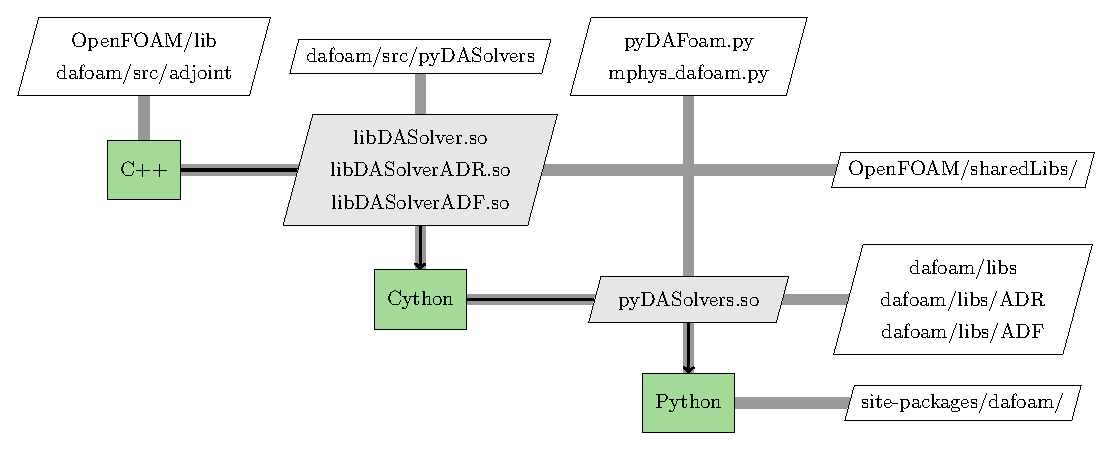
\includegraphics[width=1.18\linewidth]{images/dafoam_layers.pdf} 
\caption{There are three code layers in DAFoam: C++, Cython, and Python. Each layer takes source code or libraries as input in the vertical direction and outputs libraries to the horizontal direction.}
\end{figure}

\end{frame}
%---------------------------------------------------------------%


%---------------------------------------------------------------%
\begin{frame}[fragile]{New features in v4 layer interaction}


\begin{itemize}
  \setlength\itemsep{0.5em}
 \item We can directly pass a Python array from Python to the C++ layer. There is no need to use PETSc vectors as inputs/outputs. \href{https://github.com/mdolab/dafoam/blob/v4.0.2/src/pyDASolvers/pyDASolvers.pyx#L253}{\textcolor{blue}{[Link to an example]}}.
 \item The Python layer can call the C++ layer's members, AND the C++ layer can also call the Python layer's members. 
 \href{https://github.com/mdolab/dafoam/blob/v4.0.2/src/adjoint/DARegression/DARegression.C#L512}{\textcolor{blue}{[Link to an example]}}.
 \item The C++ layer no longer separate incompressible, compressible, and solid libs. All these flow conditions are now compiled into one library.
\end{itemize}
  
\end{frame}
%---------------------------------------------------------------%


%---------------------------------------------------------------%
\begin{frame}[fragile]{Let us build DAFoam}


\begin{itemize}
  \setlength\itemsep{0.5em}
  \item Open a terminal and cd to workshops/2025\_Summer
 \item Create a DAFoam Docker container v4.0.2. Refer to \href{https://dafoam.github.io/mydoc_get_started_run.html}{\textcolor{blue}{[this page]}} for the commands.
 \item In the container, cd to /home/dafoam/repos/dafoam, and run
 \begin{lstlisting}
./Allmake
 \end{lstlisting}
 \item That is it. The Docker image has a pre-compiled dafoam v4.0.2, so the above command will only verify the pre-compiled version and will take less than 30 seconds. At the end of the terminal output, you should see: "Build Successful!"
 \item NOTE: If you modify DAFoam and want to rebuild it, simply run the above command again. DO NOT run Allclean. DAFoam will automatically compile \textbf{only} the new files you change. This saves a lot of time!
\end{itemize}
  
\end{frame}
%---------------------------------------------------------------%


%---------------------------------------------------------------%
\begin{frame}{How to add new features in DAFoam v4?}
  Outline
  \begin{itemize}
  \item Change existing functions/variables in the C++ layer
  \item Add a new parameter in DAOption
  \item Add a new C++ function and expose it to the Python layer
  \item Add a new objective/constraint function
  \item Add a new design variable or input
  \item Add new coupling variables for MDO
  \item Add a new boundary condition
  \item Add a new turbulence model
  \item Add a new solver

\end{itemize}
\end{frame}
%---------------------------------------------------------------%

%---------------------------------------------------------------%
\begin{frame}[fragile]{Change existing functions/variables in the C++ layer}

\begin{itemize}
  \item cd into \$HOME/dafoam/repos/dafoam/
  \item Use the vi command to open the src/adjoint/DASolver/DASimpleFoam/DASimpleFoam.C file
  \item Add a print statement at the end of the solverPrimal function
 \begin{lstlisting}
Info << "This is my first change!" << endl;
 \end{lstlisting}
  \item Recompile DAFoam (make sure you see "Build Successful!"):
 \begin{lstlisting}
./Allmake
 \end{lstlisting}
  \item cd into \$HOME/mount/examples/NACA0012
  \item Run:
\begin{lstlisting}
chmod -R 750 *
./preProcessing.sh
python runScript_v4.py -task=run_model
\end{lstlisting}
 \item Verify if you see the new print statement in the terminal output
    
\end{itemize}

\end{frame}
%---------------------------------------------------------------%


%---------------------------------------------------------------%
\begin{frame}[fragile]{Add a new parameter in DAOption (1/2)}

\begin{itemize}
  \item cd into \$HOME/dafoam/repos/dafoam/
  \item Use the vi command to open the dafoam/pyDAFoam.py file and add this to the \_\_init\_\_ function of the DAOPTION class:
 \begin{lstlisting}
self.testOption = 3.0
 \end{lstlisting}
 \item NOTE: We need to give default values for str, int, float, and list options defined here (this helps DAFoam determine the datatype). For dict options, we can leave it blank.
 \item Open src/adjoint/DASolver/DASimpleFoam/DASimpleFoam.C and add this line at the end of the solverPrimal function
 \begin{lstlisting}
scalar testOption = 
    daOptionPtr_->getOption<scalar>("testOption");
Info << "My test option is: " << testOption << endl;
 \end{lstlisting}
 \item Recompile DAFoam

\end{itemize}

\end{frame}
%---------------------------------------------------------------%


%---------------------------------------------------------------%
\begin{frame}[fragile]{Add a new parameter in DAOption (2/2)}

\begin{itemize}
 \item In \$HOME/mount/examples/NACA0012, run
\begin{lstlisting}
python runScript_v4.py -task=run_model
\end{lstlisting}
  \item Verify if you see the new testOption value (3.0; default value) in the terminal output
  \item You can also change the default value in the runScript.py. For example, you can add the following line to the daOption dict in \$HOME/mount/examples/NACA0012/runScript\_v4.py.
 \begin{lstlisting}
"testOption": 15.2,
 \end{lstlisting}
\item Run the following again and see if the testOption's value is changed to 15.2 in the terminal output.
\begin{lstlisting}
python runScript_v4.py -task=run_model
\end{lstlisting}
\item NOTE: The daOption defined in runScript.py will be passed to the C++ layer \textbf{only once} (when the DAFoam is initialized). If you need to pass the daOption from Python to C++ again, you need to manually call updateDAOption(). Here is \href{https://github.com/mdolab/dafoam/blob/27d7279e32e62fa2c65399f3441836aefc8401c5/dafoam/pyDAFoam.py#L825}{\textcolor{blue}{[an example]}}.
\end{itemize}

\end{frame}
%---------------------------------------------------------------%


%---------------------------------------------------------------%
\begin{frame}[fragile]{Add a C++ func and expose it to the Python layer (1/2)}

\begin{itemize}
  \item cd into \$HOME/dafoam/repos/dafoam/, open src/adjoint/DASolver/DASolver.H, and add a public member:
 \begin{lstlisting}
void printMeshSize() 
{
    label nCells = meshPtr_->nCells();
    Info << "Mesh cells: " << nCells << endl;
}
 \end{lstlisting}
  \item Open src/pyDASolvers/DASolvers.H, and add a public member:
 \begin{lstlisting}
void printMeshSize()
{
    DASolverPtr_->printMeshSize();
}
 \end{lstlisting}
  \item Open src/pyDASolvers/pyDASolvers.pyx, and add this to \texttt{cppclass DASolvers}:
 \begin{lstlisting}
void printMeshSize()
 \end{lstlisting}
\end{itemize}

\end{frame}
%---------------------------------------------------------------%

%---------------------------------------------------------------%
\begin{frame}[fragile]{Add a C++ func and expose it to the Python layer (2/2)}

\begin{itemize}
  \item Open src/pyDASolvers/pyDASolvers.pyx,  and add this to \texttt{cdef class pyDASolvers:}
 \begin{lstlisting}
def printMeshSize(self):
    self._thisptr.printMeshSize()
 \end{lstlisting}
 \item Open dafoam/pyDAFoam.py and add this line to the end of the \_\_call\_\_ function
  \begin{lstlisting}
self.solver.printMeshSize()
 \end{lstlisting}
 \item Recompile DAFoam
 \item In \$HOME/mount/examples/NACA0012, run the following, and you should see the printed statement from the terminal output
 \begin{lstlisting}
python runScript_v4.py -task=run_model
\end{lstlisting}
\item Alternatively, you can call this new function in runScript\_v4.py by adding this line after \texttt{prob.run\_model()}
 \begin{lstlisting}
print("Print in the runScript")
prob.model.scenario1.coupling.solver.DASolver.solver.printMeshSize()
\end{lstlisting}
\end{itemize}

\end{frame}
%---------------------------------------------------------------%

%---------------------------------------------------------------%
\begin{frame}[fragile]{Add a new objective/constraint function (1/2)}

\begin{itemize}
  \item cd into src/adjoint/DAFunction
  \item Copy DAFunctionPatchMean.C into DAFunctionTestFunc.C and copy DAFunctionPatchMean.H into DAFunctionTestFunc.H
  \item Open DAFunctionTestFunc.C and replace all "DAFunctionPatchMean" with "DAFunctionTestFunc". Do the same for DAFunctionTestFunc.H
  \item (Important!) Replace TypeName("patchMean") with TypeName("testFunc") in DAFunctionTestFunc.H. Here, TypeName defines the function name we will use in runScript.py
  \item Modify DAFunctionTestFunc.C and DAFunctionTestFunc.H as needed to compute and return the function value in calcFunction(). Ensure that the function value is summed across all processors. (Call the \texttt{reduce} command).
  \item Add a print statement at the end of the calcFunction() function, which will be used to verify the implementation.
    \begin{lstlisting}
Info << "This is my test function " << endl;
 \end{lstlisting}
 \item Add DAFunction/DAFunctionTestFunc.C to src/adjoint/Make/files

\end{itemize}

\end{frame}
%---------------------------------------------------------------%


%---------------------------------------------------------------%
\begin{frame}[fragile]{Add a new objective/constraint function (2/2)}

\begin{itemize}
  \item Recompile DAFoam
  \item In \$HOME/mount/examples/NACA0012/runScript\_v4.py, add these lines to the \texttt{function} dict from daOption.
  \begin{lstlisting}
 "Test": {
    "type": "testFunc",
    "source": "patchToFace",
    "patches": ["wing"],
    "varName": "p",
    "varType": "scalar",
    "index": 0,
    "scale": 1.0},
 \end{lstlisting}
  \item Then, run the following, and you should see the function value and custom print statement in the terminal output.
 \begin{lstlisting}
python runScript_v4.py -task=run_model
\end{lstlisting}
\item NOTE: DAFoam will take care of the derivative computation for this new function automatically.
\end{itemize}

\end{frame}
%---------------------------------------------------------------%


%---------------------------------------------------------------%
\begin{frame}[fragile]{Add a new design variable or input (1/2)}

\begin{itemize}
  \item cd into src/adjoint/DAInput
  \item Copy DAInputPatchVelocity.C into DAInputPatchVx.C and copy DAInputPatchVelocity.H into DAInputPatchVx.H
  \item Open DAInputPatchVx.C and replace all "DAInputPatchVelocity" with "DAInputPatchVx". Do the same for DAInputPatchVx.H
  \item (Important!) Replace TypeName("patchVelocity") with TypeName("patchVx") in DAInputPatchVx.H.
  \item Modify DAInputPatchVx.C and  DAInputPatchVx.H as needed to assign the Vx value from input[0] to the OpenFOAM's U field.
  \item Change "return 2" to "return 1" for the size() func in DAInputPatchVx.H
  \item Add DAInput/DAInputPatchVx.C to src/adjoint/Make/files
  \item Recompile DAFoam
  \item NOTE: that is all the changed needed to add a new design variable, the rest of the operations, such as computing the partial derivatives dF/dX or dR/dX, will be automatically handled

\end{itemize}

\end{frame}
%---------------------------------------------------------------%

%---------------------------------------------------------------%
\begin{frame}[fragile]{Add a new design variable or input (1/2)}

\begin{itemize}
  \item In \$HOME/mount/examples/xxxx/runScript.py, add these lines to the \texttt{inputInfo} dict from daOption.
  \begin{lstlisting}
 "vx_in": {
    "type": "patchVx",
    "patches": ["inlet"],
    "components": ["solver", "function"]},
 \end{lstlisting}
 \item In the same runScript, add these lines to the \texttt{configure} function.
\begin{lstlisting}
self.dvs.add_output("vx_in", val=np.array([10.0]))
self.connect("vx_in", "scenario1.vx_in")
self.add_design_var("vx_in", upper=50.0, scaler=1.0)
 \end{lstlisting}
\item Finally, run the following, and verify the inlet velocity in Paraview
 \begin{lstlisting}
python runScript.py -task=run_model
\end{lstlisting}
\item You can also change the default value from 10 to 20 in the \texttt{self.dvs.add\_output} call, run the script again, and then verify the new inlet value in Paraview
\end{itemize}

\end{frame}
%---------------------------------------------------------------%


%---------------------------------------------------------------%
\begin{frame}[fragile]{Add a new boundary condition}

\begin{itemize}
  \item Copy a template of the boundary condition .C and .H files from OpenFOAM and paste them to src/adjoint/DAMisc/.
  \item Modify the .C and .H file as needed. Remember to change TypeName("your\_new\_bc\_name") in the .H file to a custom name that has not been used in OpenFOAM.
  \item Add the .C file's path to src/adjoint/Make/files
  \item Recompile DAFoam
  \item You can use your new boundary condition now. Remember to use your custom name.
\end{itemize}

\end{frame}
%---------------------------------------------------------------%

%---------------------------------------------------------------%
\begin{frame}[fragile]{Add a new turbulence model (1/2)}

\begin{itemize}
  \item Copy the turbulence model .C and .H files from OpenFOAM and paste (use custom names like mySA.C and mySA.H) them to src/newTurbModels/models.
  \item Replace the old turbulence class name with your new turbulence name. Don't forget to assign a custom name for the TypeName in the .H file.
  \item The turbulence model here is used to initialize the parent class and turbulence variable. So we need do delete all intermediate functions or variables and keep only these things: (1) The initialization of eddyViscosity and turbulence variables, such as nuTilda\_, k\_, omega\_. (2) All the virtual function, (3) An empty correct() function.
  \item In src/newTurbModels/compressible, copy makeSpalartAllmarasFv3Compressible.C and paste it into sth like makeMySAModelCompressible.C. Then, in makeMySAModelCompressible.C, replace  SpalartAllmarasFv3 with your custom turbulence name. Finally, add makeMySAModelCompressible.C to src/newTurbModels/compressible/Make/files
\end{itemize}

\end{frame}
%---------------------------------------------------------------%

%---------------------------------------------------------------%
\begin{frame}[fragile]{Add a new turbulence model (2/2)}

\begin{itemize}
  \item Do the same to create makeMySAModelIncompressible.C file in src/newTurbModels/incompressible
  \item In addition to the dummy turbulence initialization class above, we need to add the actual turbulence model computation to the DATurbulenceModel class.
  \item First, in /src/adjoint/DAModel/DATurbulenceModel, copy DASpalartAllmaras.C and DASpalartAllmaras.H and paste them to custom names.
  \item Replace the old turbulence class name with your new turbulence name. Don't forget to assign a custom name for the TypeName in the .H file.
  \item Modify the the custom .C and .H files as needed. Follow the code structure from existing model implementations. The actual solution of the turbulence model should be implemented in the calcResiduals() function.
  \item Add your custom .C file's path to src/adjoint/Make/files
  \item Recompile DAFoam, and your new turbulence model is ready to use.
\end{itemize}

\end{frame}
%---------------------------------------------------------------%


%---------------------------------------------------------------%
\begin{frame}[fragile]{Add new coupling variables for MDO (1/2)}

\begin{itemize}
  \item In MDO, we often need to extract boundary variables from the solver and pass these variables to another solver. Examples include the surface force for aero-structural coupling and the surface temperature for aero-thermal coupling. 
  \item Here we go over the process of extracting surface nodal force for aero-structural coupling.
  \item First, we need to add a child class (DAOutputForceCoupling) to src/adjoint/DAOutput.
  \item In DAOutputForceCoupling.H, we need to define the size of the surface nodal force, and set distributed to 1, meaning each processor owns and extracts their own surface nodal force values.
  \item In DAOutputForceCoupling.C, we need to implement how to extract the surface nodal force values, and then assign them to the \texttt{output} variable in the \texttt{run} function.
  \item This output is ready to use in the Python layer.
\end{itemize}

\end{frame}
%---------------------------------------------------------------%


%---------------------------------------------------------------%
\begin{frame}[fragile]{Add new coupling variables for MDO (2/2)}

\begin{itemize}
  \item Next, we need to add a new explicit component called DAFoamForces to dafoam/mphys/mphys\_dafoam.py. This component's inputs are the states and volume coordinate, and the output is the surface nodal forces.
  \item The compute method in the DAFoamForces component calls the calcOutput() function to extract the nodal forces and assign them to the forces array. The outputName and outputType are defined in outputInfo in runScript.py
  \item The compute\_jacvec\_product method in DAFoamForces component calls the calcJacTVecProduct() function to compute partial derivatives 
\end{itemize}

\end{frame}
%---------------------------------------------------------------%


\end{document}

